\chapter{Introduzione}
\label{cap:int}
\section{Cos'è un Tema Natale?}
Un \textbf{Tema Natale} è una disposizione irripetibile di elementi astrologici, i quali comprendono Segni, Case e Pianeti.\newline
In realtà esistono soltanto circa tre dozzine di parole nel vocabolario astrologico, ma collegandole tutte tra loro, le combinazioni risultanti diventano praticamente infinite.\newline
Un Tema Natale è una di quelle particolari e quasi irripetibile combinazioni che rappresenta un singolo individuo.\newline
Fisicamente, un Tema Natale è semplicemente una mappa. Essa mostra il modo in cui i \textbf{Pianeti} erano disposti nel cielo al momento della nascita di una persona.\newline
I geroglifici sparsi a caso lungo tutta la mappa rappresentano il Sole, la Luna e tutti gli altri pianeti.\newline
\begin{figure}[H]
\centering
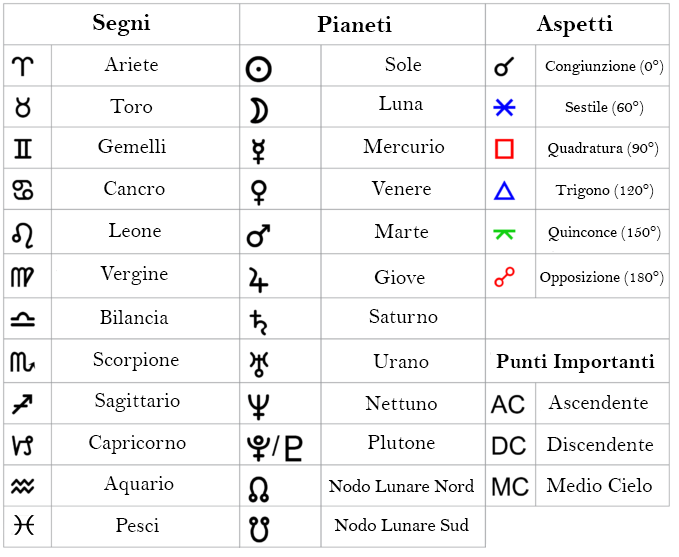
\includegraphics[width=\textwidth, height=0.35\textheight, keepaspectratio]{img/glyph.png}
\caption{Glifi di Segni, Pianeti, Aspetti e Punti Importanti}
\label{fig:glyph}
\end{figure}

Questi simboli vengono chiamati glifi. Anche i segni zodiacali, come i pianeti, hanno dei glifi. I glifi più famosi ed importanti sono riportati in Figura \ref{fig:glyph} (si noti che in astrologia, Sole, Luna e Plutone sono considerati Pianeti).\newline
Riportiamo il Tema Natale di esempio, di una persona nata il 10 Dicembre 1998, a Fano (PU/ Marche/ Italia) alle 20:13 (ora locale italiana) in Figura \ref{fig:natal}.\newline
\begin{figure}[H]
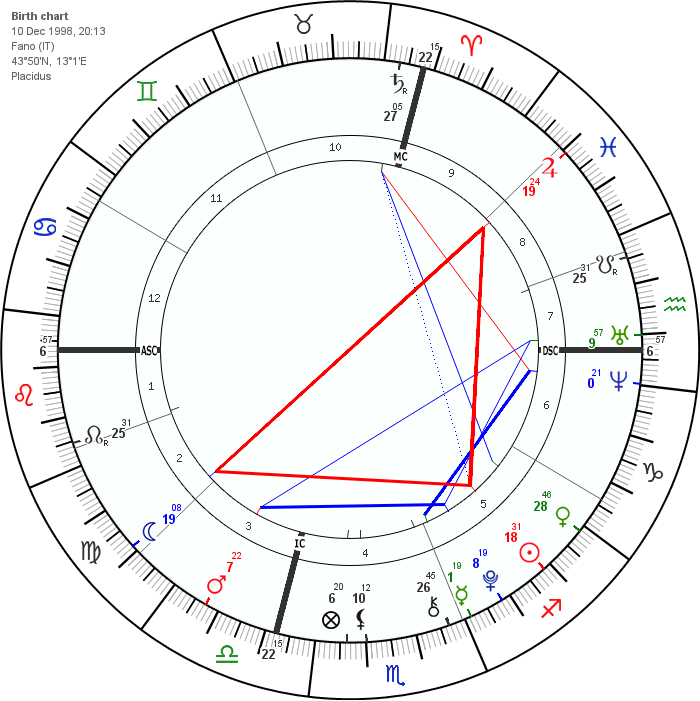
\includegraphics[width=\textwidth,height=\textheight,keepaspectratio]{img/natal.png}
\caption{Un esempio di Tema Natale}
\label{fig:natal}

\end{figure}
La linea orizzontale che corre lungo la parte di mezzo del nostro Tema d'esempio è l'orizzonte locale.\newline
Tutto ciò che si trova sopra quella linea era nella parte visibile del cielo al momento della nascita di quell'Individuo.\newline
Tutto ciò che si trova sotto era invece invisibile, nascosto dall'altra parte della Terra.\newline
La parte sinistra di quella linea rappresenta l'Est (solo i due poli Est e Ovest sono invertiti).\newline
A Dicembre, in Italia, il sole è tramontato da qualche ora, ed infatti vediamo che il glifo del Sole (il cerchio con un punto al centro) è collocato, molto sotto la linea del tramonto (quella ad Ovest), proprio dove ci aspettavamo che fosse.\newline
È proprio in funzione dell'orizzonte che definiamo il concetto di \textbf{Casa}. A partire dall'Est andando in senso antiorario troviamo ordinate tutte le dodici case astrologiche, identificate da un numero.\newline
Nel nostro esempio, il sole giace nella quinta casa. Notiamo che nella stessa casa ci sono anche altri pianeti, Mercurio, Venere e Plutone. Se ci muoviamo più all'esterno troviamo i dodici \textbf{Segni Zodiacali}. Inizialmente, molte persone tendono a confondere i segni con le case, ma è importante tenere i due concetti separati nella propria mente; le case sono collegate all'orizzonte mentre i segni allo Spazio. Dato che la Terra ruota nello Spazio, i Segni sembrano girare attorno alla Terra.\newline
Ogni Pianeta cade sia in un Segno che in una Casa. Nel nostro esempio il sole si trova in Sagittario, così come tutti gli altri pianeti della stessa casa. Osserviamo però Urano e Nettuno: essi si trovano nello stesso segno ma in case diverse.\newline
Ogni pianeta rappresenta una precisa funzione psicologica umana. Mettendo insieme tutti i pianeti otterremmo una dettagliata mappa della psiche umana. I segni simboleggiano processi che accadono all'interno della mente. Ognuno dei dodici ha obiettivi diversi, risorse diverse, caratteristiche uniche.
Le case, sono molto più concrete, in quanto non sono altro che palcoscenici, aree della vita con cui abbiamo a che fare tutti i giorni.\newline
Abbiamo poi gli \textbf{Aspetti}: fisicamente, non sono altro che angoli geometrici tra pianeti e altri punti.\newline
Nei secoli però, si è scoperto che alcuni angoli tendono a creare particolari interazioni. In pratica, due pianeti legati da un'aspetto interagiscono tra loro in qualche modo, influenzandosi l'un l'altro. In figura \ref{fig:natal}, gli aspetti sono le linee che troviamo nel cerchio più interno. Il più delle volte, non essenso molto chiaro questo metodo di rappresentazione, si tende a preferire la vista degli aspetti in una tabella come quella in Figura \ref{fig:aspect}.
\begin{figure}[H]
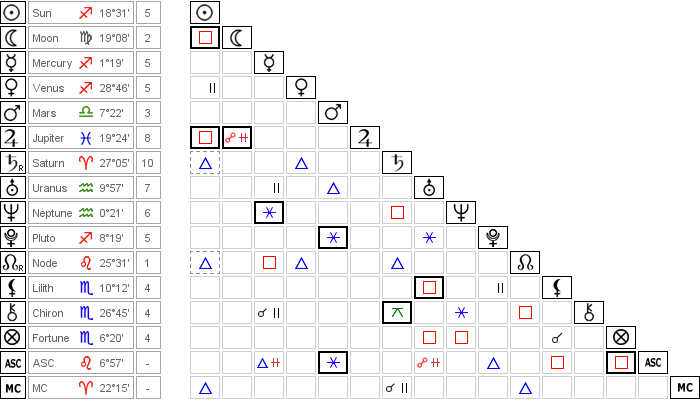
\includegraphics[width=\textwidth,height=\textheight,keepaspectratio]{img/aspect.png}
\caption{Tabella degli aspetti}
\label{fig:aspect}
\end{figure}
Punti molto importanti infine, sono gli estremi dell'orizzonte e del cielo. Ad Est troviamo l'\textbf{Ascendente}, ad Ovest il \textbf{Discendente}. Il punto più alto del cielo viene chiamato appunto \textbf{Medio Cielo} e il suo opposto, dall'altra parte della terra si chiama \textbf{Fondo Cielo} o \textbf{Nadir}. Questi punti coincidono sempre con l'inizio di una casa specifica, la prima per l'Ascendente, la settima per il Discendente, la decima per il Medio Cielo e la quarta per il Nadir.\newline
Se conosciamo il segno che cade nell'Ascendente, abbiamo gratis il segno del Discendente, in quanto ogni segno ha un suo opposto. Non possiamo però sapere con certezza il segno che cade nel Medio Cielo sapendo il segno dell'Ascendente, perchè i segni occupano esattamente 30 gradi ciascuno nella ruota, ma le case sono variabili e possono anche occupare più di 30 gradi o anche meno.
In pratica, il punto più alto del Cielo, non é sempre a metà strada tra i due estremi Est e Ovest, proprio come capita nel Tema Natale d'Esempio.
